% vim: spelllang=es

% Instrucciones:
% https://eina.unizar.es/sites/eina.unizar.es/files/archivos/secretaria/20210706_instrucciones_tfg_tfm.pdf
%
% TFGs previos:
% https://zaguan.unizar.es/search?ln=en&cc=trabajos-fin-grado&sc=1&p=inform%C3%A1tica&f=Departamento&action_search=Search
%
% Blog:
% https://nullderef.com/series/rust-plugins/
%
% NOTES:
% * Count words with `:TexWordCount`
% * Svg to pdf: `inkscape -D image.svg  -o image.pdf --export-latex`
%
% TODO:
% * Buscar (grep) comas antes de conjunciones (y, e, o, u)
%
% * Debería tener palabras anglosajonas con `\emph` siempre?
%
% * No sé cómo traducir onramp, offramp, sink y source de forma precisa.
%
% * Debería traducir runtime por ejecutor?
%
% * Debería incluir las figuras siempre en su sitio, donde las pone LaTeX por
% defecto, o al final de la sección?

\documentclass[a4paper,12pt,twoside,hidelinks,openright]{book}

% \usepackage[T1]{fontenc}
\usepackage[spanish]{babel}
\usepackage[utf8]{inputenc}

\usepackage[usenames, dvipsnames]{color}
\usepackage{graphicx}
\usepackage{multirow}
\usepackage{graphics}
\usepackage{appendix}
\usepackage[nottoc,numbib]{tocbibind}
\usepackage{xspace}

\usepackage{tikz}
\usetikzlibrary{shapes,arrows}
\usepackage{subcaption}
\usepackage{amsmath,amsthm,amssymb,mathrsfs} 
\usepackage[final]{pdfpages}
\usepackage[]{placeins,flafter}
\usepackage[none]{hyphenat} \sloppy
\usepackage{xcolor}
\usepackage{adjustbox}
\usepackage{hyperref}

% Bibtex for the bibliography
\usepackage[
    backend=bibtex,
    block=space,
    language=spanish,
    sorting=none % Sort by appearance in the document
]{biblatex}
\bibliography{Bibliografia_TFG}

% Easier to read font
\usepackage{fourier} % For math
\usepackage{fontspec}
\setmainfont{Heuristica} % For the text
\setmonofont{Liberation Mono} % For the code

% Less margin between lists, otherwise after overriding \parskip and etc it's
% too much.
% TODO: decidir si hacer párrafos estilo TeX o convencionales.
\usepackage{enumitem}
\setlist{topsep=0pt}

% Code syntax highlighting
\usepackage{minted}
\usepackage{xcolor}
\usemintedstyle{vs}
\definecolor{bg}{HTML}{f8f8f8}
\setminted{
    frame=lines,
    framesep=2mm,
    bgcolor=bg,
    fontsize=\footnotesize,
    linenos
}

% Remove red boxes around illegal characters in minted, taken from:
% https://tex.stackexchange.com/a/343506
%
% This way, `mysql` can be used to highlight tremorscript as a quick hack.
\makeatletter
\AtBeginEnvironment{minted}{\dontdofcolorbox}
\def\dontdofcolorbox{\renewcommand\fcolorbox[4][]{##4}}
\makeatother

% Command for inline code
\newcommand{\code}[1] {\mintinline{text}{#1}}
\newcommand{\image}[1] {
  \begin{figure}[H]
    \centering
    \includegraphics[width=\textwidth]{#1}
  \end{figure}
}
% Shortcuts
\newcommand{\cpp}{C\texttt{++}}
\newcommand{\cratelink}[1] {%
    \code{#1}\footnote{\url{https://crates.io/crates/#1}}\xspace%
}
% Gracias unizar por no evolucionar y solo permitir memorias en castellano...
\newcommand{\crate}{\emph{crate}\xspace}
\newcommand{\crates}{\emph{crates}\xspace}
\newcommand{\onramp}{\emph{onramp}\xspace}
\newcommand{\onramps}{\emph{onramps}\xspace}
\newcommand{\offramp}{\emph{offramp}\xspace}
\newcommand{\offramps}{\emph{offramps}\xspace}
% TODO: sink/source sí que se podrían traducir por salida/entrada
\newcommand{\sink}{\emph{sink}\xspace}
\newcommand{\sinks}{\emph{sinks}\xspace}
\newcommand{\source}{\emph{sources}\xspace}
\newcommand{\sources}{\emph{sources}\xspace}
\newcommand{\pipeline}{\emph{pipeline}\xspace}
\newcommand{\pipelines}{\emph{pipelines}\xspace}
\newcommand{\builder}{\emph{builder}\xspace}
\newcommand{\builders}{\emph{builders}\xspace}
\newcommand{\lifetime}{\emph{lifetime}\xspace}
\newcommand{\lifetimes}{\emph{lifetimes}\xspace}
\newcommand{\websockets}{\emph{websockets}\xspace}
\newcommand{\trait}{\emph{trait}\xspace}
\newcommand{\traits}{\emph{traits}\xspace}
\newcommand{\scripting}{\emph{scripting}\xspace}

%	CONFIGURACIÓN DE PÁGINA

\setlength{\paperwidth}{21cm}          % Ancho de página
\setlength{\paperheight}{29,7cm}       % Alto de página
\setlength{\textwidth}{15.5cm}         % Ancho de zona con texto
\setlength{\textheight}{24.6cm}        % Ancho de zona con texto
\setlength{\topmargin}{-1.0cm}         % Margen superior
                                      
\setlength{\oddsidemargin}{0.46cm}     % Margen izquierdo 
\setlength{\evensidemargin}{0.46cm}    

\usepackage{makeidx}
\makeindex
\index{key}
\newcommand{\myref}[1]{\color{red}\bf(\ref{#1})}


\begin{document}

% PORTADA
\begin{titlepage}

\definecolor{unizarblue}{RGB}{0, 86, 153}

\vspace*{-4mm}
\begin{figure}[!h]
  \centering
	
\includegraphics[width=69.62mm]{Imagenes/UnizarLogo}
\end{figure}

\vspace*{17mm}

\fontsize{28pt}{28pt}\selectfont
\begin{center}
\setlength{\fboxsep}{3.4mm}
\adjustbox{minipage=14.4cm,cfbox=unizarblue,center}{\begin{center} Trabajo Fin de Grado \end{center}}
\end{center}

\vspace*{18.7mm}


\fontsize{22pt}{22pt}\selectfont
\begin{center}
\textsc{Dynamic loading of plugins in Rust \\
in the absence of a stable \\
Application Binary Interface}
\end{center}

\vspace*{1cm} 
\baselineskip 36pt
\begin{center}

\fontsize{14pt}{14pt}\selectfont
\center{\rm Autor:}
\vspace*{0mm} 
\fontsize{18pt}{18pt}\selectfont
\center{\textsc{Mario Ortiz Manero}}

\vspace*{0.5cm}
\baselineskip 36pt

\fontsize{14pt}{14pt}\selectfont
\center{\rm  Director:}
\vspace*{0mm}
\fontsize{15pt}{15pt}\selectfont
\center{\textsc{Javier Fabra Caro}}

\end{center}

\setcounter{footnote}{1}

\vspace*{35mm}
\fontsize{14pt}{14pt}\selectfont
\begin{center}
Grado en Ingeniería Informática\\ \medskip
Departamento de Ingeniería e Ingeniería de Sistemas\\
Escuela de Ingeniería y Arquitectura\\ \bigskip
Junio 2022\\
\end{center}


\renewcommand{\thefootnote}{\arabic{footnote}}
\pagenumbering{gobble}
\end{titlepage}
\newpage


\title{Dynamic loading of plugins in Rust in the absence of a stable Application Binary Interface}
\author{Mario Ortiz Manero}

\pagebreak
\cleardoublepage%
\baselineskip 19pt

\renewcommand{\labelitemi}{$-$}
\renewcommand{\tablename}{Tabla}

\renewcommand{\appendixname}{Anexos}
\renewcommand{\appendixtocname}{Anexos}
\renewcommand{\appendixpagename}{Anexos}


\pagenumbering{Roman}

% Párrafos de forma más convencional, me parece más fácil leerlo así.
\begingroup
\setlength{\parskip}{\baselineskip}%
\setlength{\parindent}{0pt}%

\newpage
\cleardoublepage%
% vim: spelllang=es

\begin{center}
{\LARGE \bfseries AGRADECIMIENTOS}
\vspace{2.5cm}
\end{center}

Un primer gracias a toda mi familia por apoyarme en cualquier momento que lo
necesitara. En especial, a mi padre y a mi madre por aguantarme siempre y por
dejarse la piel para que pueda estudiar.

A mis amigos que me han acompañado toda la vida con tan buenos momentos, y a los
de la universidad, que fueron la verdadera motivación a ir a clase y seguir día
a día. Las horas incontables juntos en la biblioteca, en el bar de la EINA o
incluso en los montes más recónditos de Juslibol a las dos de la madrugada, han
hecho que estos años merezcan la pena.

También a mis profesores por orientarme, particularmente a Javier Fabra por
ayudarme con mi Erasmus, este documento y todas sus complicaciones. Mis mentores
de Tremor tomaron un papel fundamental, no solo dándome consejo para el
proyecto, sino también para mi carrera profesional y mi vida.

Finalmente, agradecer a todas las organizaciones que han hecho esto posible. A
la Fundación de Linux por ofrecer los medios. A Wayfair por apostar sus fondos
en código abierto y talento joven. Y a la comunidad de código abierto, que me ha
motivado a programar desde el principio y me ha guiado hasta donde estoy hoy.


\newpage
\cleardoublepage%
% vim: spelllang=es

\begin{center}
{\LARGE \bfseries RESUMEN}

\vspace{2.5cm}
\end{center}

La toma de decisiones de muchas empresas modernas como Wayfair se basa en la
recolección y análisis de datos de sus sistemas. Para llevarlo a cabo de forma
eficiente en una escala masiva, es necesario el uso de herramientas de alto
rendimiento como Tremor, escrito con Rust, programación asíncrona y SIMD.

A medida que Tremor evoluciona, sus tiempos de compilación crecen y,
consecuentemente, se deteriora la experiencia de desarrollo. Esto se puede
aliviar implementando un sistema de plugins que divide su único binario en
componentes más pequeños compilables independientemente.

Existen múltiples tecnologías disponibles para su desarrollo: lenguajes
interpretados, WebAssembly, eBPF, comunicación inter-proceso o cargado dinámico.
Sin embargo, gran parte de ellas deben descartarse por no cumplir los estándares
de eficiencia de Tremor. Entre las alternativas restantes, se escoge cargado
dinámico por ser la más usable y popular.

El cargado dinámico es imposible con tipos y funciones declarados con Rust puro,
ya que su Interfaz Binaria de Aplicación (ABI) no es estable. Será necesario
convertir los tipos al ABI de C, que sí es estable, y viceversa. Para facilitar
el proceso, se pueden aprovechar librerías existentes y herramientas del
lenguaje como macros procedurales.

Dado que el cargado dinámico en Rust es un ecosistema muy nuevo, es necesario
contribuir en código abierto a gran cantidad de sus dependencias para
implementar la funcionalidad necesaria para un sistema de plugins.

La complejidad del proyecto incrementó significativamente respecto al plan
original, por lo que aunque funcional, no alcanza alguno de los objetivos
iniciales, principalmente relacionados con el rendimiento. Sin embargo, sirve
como una buena base para futuras versiones de Tremor que sí que lo incluyan en
producción, y continuará evolucionando con el programa.


\newpage
\cleardoublepage%
% vim: spelllang=en

\begin{center}
{\LARGE \bfseries ABSTRACT}

\vspace{2.5cm}
\end{center}


Una mañana, tras un sueño intranquilo, Gregorio Samsa se despertó convertido en un monstruoso insecto. Estaba echado de espaldas sobre un duro caparazón y, al alzar la cabeza, vio su vientre convexo y oscuro, surcado por curvadas callosidades, sobre el que casi no se aguantaba la colcha, que estaba a punto de escurrirse hasta el suelo. Numerosas patas, penosamente delgadas en comparación con el grosor normal de sus piernas, se agitaban sin concierto. - ¿Qué me ha ocurrido? No estaba soñando. Su habitación, una habitación normal, aunque muy pequeña, tenía el aspecto habitual. Sobre la mesa había desparramado un muestrario de paños - Samsa era viajante de comercio-, y de la pared colgaba una estampa recientemente recortada de una revista ilustrada y puesta en un marco dorado. La estampa mostraba a una mujer tocada con un gorro de pieles, envuelta en una estola también de pieles, y que, muy erguida, esgrimía un amplio manguito, asimismo de piel, que ocultaba todo su antebrazo. Gregorio miró hacia la ventana; estaba nublado, y sobre el cinc del alféizar repiqueteaban las gotas de lluvia, lo que le hizo sentir una gran melancolía. «Bueno -pensó-; ¿y si siguiese durmiendo un rato y me olvidase de

\endgroup

\newpage
\cleardoublepage%
\renewcommand{\contentsname}{Índice}
\tableofcontents

% Capitulos

% Vuelta a configurar los párrafos para que no afecte al índice
\setlength{\parskip}{\baselineskip}%
\setlength{\parindent}{0pt}%

% vim: spelllang=es

\chapter{Introducción}
\pagenumbering{arabic}

\section{Contexto}

% TODO: quizá algunos footnotes podrían cambiarse por referencias aquí
Este proyecto se ha realizado en colaboración con
\emph{Tremor}\footnote{\url{https://tremor.rs}}, un sistema de procesado de
eventos de alto rendimiento, escrito en el lenguaje de programación
\emph{Rust}\footnote{\url{https://www.rust-lang.org}}. Tremor es un programa de
código abierto bajo la fundación \emph{Cloud Native Computing
Foundation~(CNCF)}\footnote{\url{https://www.cncf.io/}}, que es también parte de
la organización \emph{Linux
Foundation~(LFX)}\footnote{\url{https://www.linuxfoundation.org/}}.

Formalmente, el trabajo se ha llevado a cabo gracias a la iniciativa \emph{LFX
Mentorship}, con el título ``CNCF -- Tremor: Add plugin support for tremor
(PDK)''\footnote{Página oficial de la iniciativa:
\url{https://mentorship.lfx.linuxfoundation.org/project/b90f7174-fc53-40bc-b9e2-9905f88c38ff}}\footnote{\emph{Tracking
issue} en GitHub:
\url{https://github.com/tremor-rs/tremor-runtime/issues/791}}\footnote{RFC en la
documentación de Tremor:
\url{https://www.tremor.rs/rfc/accepted/plugin-development-kit/}}. Esta
iniciativa promueve el aprendizaje de desarrolladores de código abierto,
proporcionando una plataforma transparente y facilitando un sistema de pagos.

Finalmente, \emph{Wayfair} es una empresa estadounidense de comercio digital de
muebles y artículos del hogar\footnote{\url{https://www.wayfair.com/}}.
Actualmente, ofrece 14 millones de ítems de más de 11.000 proveedores
globales~\cite{wayfairItems} y es el principal financiador tanto de Tremor como
de este proyecto.

\section{Objetivo}

La tarea a llevar a cabo es la implementación de un sistema de plugins,
denominado \emph{Plugin Development Kit~(PDK)}, para la base de código ya
existente en Tremor.

Esto es una tarea no-trivial, dado que Rust no tiene un \emph{Application Binary
Interface~(ABI)} estable. Es decir, que si se compila la \emph{runtime} (el
binario principal encargado de cargar funcionalidad externa) y los
\emph{plugins} (los binarios individuales con la funcionalidad) de forma
separada, no hay garantía de que la representación binaria de los datos o la
convención de llamada a funciones --- entre otros --- sea la misma.

Esto implica que \emph{dynamic loading} es imposible de forma segura puramente
con Rust, debiéndose recurrir a otro ABI que sí sea estable, como el del
lenguaje de programación C. Por tanto, se deben escribir \emph{bindings} (la
definición de la interfaz compartida entre runtime y plugins) completas en C y
transformar tipos de Rust a C y viceversa cuando se interactúe con plugins.

\section{Motivación}

\subsection{Tiempos de compilación}

% TODO: incluir modo release?
Actualmente, el problema más importante en Tremor es sus tiempos de compilación.
En un ordenador de gama media de \~{}600 € como el Dell Vostro 5481, compilar el
binario \code{tremor} desde cero requiere de más de 7 minutos en modo debug.
Incluso en el caso de cambios incrementales (una vez las dependencias ya han
sido compiladas), hay que esperar unos 10 segundos. Esto no es una buena
experiencia de desarrollo e impide que nuevos programadores se unan a la
comunidad de Tremor.

Debido a la naturaleza del programa, este problema solo empeorará con el tiempo.
Tremor debe tener soporte para un gran número de protocolos (e.g., TCP o UDP),
software (e.g., Kafka o PostgreSQL) y codecs (e.g., JSON o YAML). El número de
dependencias continuará incrementando hasta que imposibilite la creación de
nuevas prestaciones en Tremor.

Los problemas relacionados con tiempos de compilación excesivamente largos no se
limitan a Tremor. Es uno de las mayores críticas que recibe Rust y un 61\% de
sus usuarios declaran que aún se necesita trabajo para mejorar la
situación~\cite{rustsurvey}.

\subsection{Modularidad}

Otra ventaja que provee un sistema de plugins es modularidad; ser capaz de
tratar la runtime y los plugins de forma separada suele resultar en una
arquitectura más limpia~\cite{baldwin2000design}. También hace posible el
desacoplamiento del ejecutable y sus componentes; algunas dependencias tienen un
ciclo de versionado más rápido que otras y generalmente es más conveniente
actualizar únicamente un plugin, en lugar del programa por completo.

\subsection{Aprender de otros}

Otros proyectos maduros con características similares a las de Tremor, como
\textcite{nginx} o \textcite{apachehttpserver}, llevan beneficiándose de un
sistema de plugins desde hace mucho. Informan mejorías en flexibilidad,
extensibilidad y facilidad de
desarrollo~\cite{nginxPluginsAdvantages}\cite{apachePluginsAdvantages}. Aunque
las desventajas también mencionen un pequeño impacto en el rendimiento y la
posibilidad de caer en un \emph{dependency hell}, sigue siendo una buena idea al
menos considerarlo para Tremor.

\section{Metodología}

\subsection{Organización}

El proyecto ha tenido una duración de unos 10 meses, comenzando en agosto de
2021 y terminando en mayo/junio de 2022. Su realización ha sido completamente
remota y con horarios muy flexibles. Se usó el servidor de Discord de
Tremor\footnote{\url{https://discord.com/invite/Wjqu5H9rhQ}} como plataforma
principal para comunicarse, tanto por texto como por videollamada. Se programó
una llamada por semana, en la que explicaba mi progreso y recibía ayuda de mis
mentores en caso de que me hubiera quedado atascado en algún momento.

% TODO: update Matthias' title
Disponía de tres mentores, que me guiaban en el proceso de desarrollo: Darach
Ennis (\emph{Principal Engineer and Director of Tremor Project}), Matthias Wahl
(\emph{Staff Engineer}) y Heinz N. Gies (\emph{Senior Staff Engineer}), todos
empleados por Wayfair.

La organización de forma más estructurada para las tareas que tenía pendientes,
en las que estaba trabajando en ese momento, y las que ya había realizado, se
basó principalmente en un Kanban en
GitHub\footnote{\url{https://github.com/marioortizmanero/tremor-runtime/projects/1}}.

\subsection{Desarrollo}

Para reducir el coste de desarrollo y asegurarse de que el proceso sea
completamente seguro (en memoria y concurrencia), el sistema de plugins
aprovecha librerías existentes en Rust y herramientas como macros procedurales.
El sistema de compilación usado es solución oficial de Rust: Cargo, que también
incluye un \emph{formatter}, \emph{linter}, y extensiones instalables creadas
por la comunidad. Adicionalmente, existe una gran cantidad de tests y
\emph{benchmarks} que se han de tener en cuenta para mantener el \emph{Code
Coverage} (la cantidad de código cubierta por los tests) y el rendimiento.

\subsection{Recursos públicos}

% TODO: actualizar '5' cuando suba el nuevo
% TODO: actualizar minutos de lectura
% TODO: al terminar, mencionar qué no se incluye aquí de los blogs
% TODO: buscar otra métrica que no sean horas de lectura, no creo que sea buena
% manera de venderlo
Este trabajo está disponible públicamente al completo. Además, a medida que he
investigado e implementado el sistema de plugins, he ido escribiendo todo en mi
blog personal, \emph{NullDeref}; gran parte de los contenidos de este documento
se han obtenido de ahí. Tiene una serie con un total de 5 artículos que entran
en gran detalle y suman unas 2 horas adicionales de lectura.

\begin{itemize}
    \item El repositorio de GitHub para el binario de Tremor:\\
        \url{https://github.com/tremor-rs/tremor-runtime}
    \item Mi \emph{fork}, con ramas adicionales usadas durante el desarrollo:\\
        \url{https://github.com/marioortizmanero/tremor-runtime}
    \item Mi repositorio con experimentos antes de implementar la versión
        definitiva:\\
        \url{https://github.com/marioortizmanero/pdk-experiments}
    \item La serie de artículos en mi blog personal:\\
        \url{https://nullderef.com/series/rust-plugins/}.
\end{itemize}

TODO: debería ser más específico sobre las horas? Mucha cuenta no he llevado
pero vamos sí que estoy segurísimo de que han sido 300 horas y mucho más
también.

TODO: debería incluir que atendí a KubeCon 2022 gracias a Tremor, explicándolo
un poco en un anexo?

TODO: quizá hacer una tabla que relacione cada sección del índice con los
capítulos relacionados de nullderef? Pero eso ya lo pondría en un anexo.

% vim: spelllang=es

\chapter{Breve introducción a Rust}\label{ch:rust}

Dado que Rust es un lenguaje de programación que tan solo anunció su primera
versión en 2015, aún no es conocido por muchos desarrolladores. Este proyecto
requiere ser familiar con cómo funciona, por lo que en este capítulo se
introducirán los conceptos más básicos necesarios. Sí que se asume conocimiento
de lenguajes de propósito general, como C, C++, Python o Java.

Sin embargo, es posible que se omitan algunos conceptos o que algunas
explicaciones no sean completamente precisas por razones de simplicidad.
\textcite{rustfullbook} es el libro oficial para aprender Rust por completo,
pero es una lectura larga y posiblemente demasiado exhaustiva. Para mayor
brevedad, se recomienda leer \textcite{rustprofessionals},
\textcite{rustgentleintro} o \textcite{rust30min}.

La comunidad dispone de otros libros que explican aspectos más avanzados del
lenguaje en específico, como \unsafe o la programación asíncrona. En esos casos,
se recomienda leer \textcite{rustnomicon} y \textcite{rustasyncbook},
respectivamente.

TODO: revisar traducciones del libro o similares para asegurarse de que la
terminología es la misma.

\section{¿Qué es Rust?}

Rust es un lenguaje de programación de sistemas compilado y de propósito
general. Su objetivo es maximizar rendimiento y usabilidad, esto último
basándose en seguridad integrada en el lenguaje, en vez de en el \

\section{Primeros pasos}

Comenzando por el clásico ``Hola Mundo'', se incluyen algunos ejemplos de cómo
es la sintaxis de Rust más básica. El programa se podría ejecutar fácilmente con
\emph{Cargo}, el administrador de dependencias oficial, o específicamente con el
comando \code{cargo run}.

\begin{minted}{rust}
fn main() {
    println!("Hello World!");
}
\end{minted}

\code{main} es nuestra función principal, que invoca al macro \emph{println}
para escribir por pantalla. Esto se sabe porque, a diferencia de una llamada a
función, la invocación termina con una exclamación (\code{!}).

Los bloques básicos (\code{if}, \code{else}, \code{while}, \code{for}) son los
mismos que en otros lenguajes, con la introducción de \code{match}, que permite
extraer patrones.

\begin{minted}{rust}
fn factorial(i: u64) -> u64 {
    match i {
        0 => 1,
        n => n * factorial(n-1)
    }
}
\end{minted}

\section{Librería estándar}

De forma similar a C++, Rust posee tipos genéricos. Esto permite la
implementación de una librería estándar flexible, con varias estructuras de
datos importantes a conocer:

\begin{itemize}
    \item Tipos primitivos:
        \begin{itemize}
            \item Carácteres con \code{char}.

            \item Punto flotante con \code{f32} y \code{f64}.

            \item Booleanos con \code{bool}.

            \item Enteros: \code{u8}, \code{i8}, \code{u16}, \code{i16},
                \code{u32}, \code{i32}, \code{u64}, \code{i64}, e incluso
                \code{i128} y \code{u128} en las arquitecturas que lo soportan.

            \item Vectores de tamaño fijo: por ejemplo \code{[1, 2, 3, 4, 5]}.

            \item N-tuplas como \code{(1, true, 9.2)}.

            \item El tipo ``unidad'', \code{()}, equivalente a \code{void} en C
                o C++.

            \item Punteros básicos con \code{*const T} o \code{*mut T}.

        \end{itemize}

    \item \code{Vec<T>} representa un vector contiguo y redimensionable.

    \item \code{HashMap<K, V>} es una tabla hash, genérica respecto a su clave
        \code{K} y su valor \code{V}. No se encuentra en el preludio, por lo que
        requeriría la siguiente declaración, similar a un \code{import} de Java:

\begin{minted}{rust}
use std::collections::HashMap;
\end{minted}

    \item \code{Box<T>}, usado para localizar un tipo \code{T} en memoria.
        Incluye el tamaño que ocupa \code{T}.

    \item \code{str} es una cadena UTF-8 de solo lectura, típicamente usada con
        una referencia \code{&str}. Va acompañada por su longitud, por lo que no
        hace falta terminarla con \code{\0}, a diferencia de C. \code{String} es
        su versión modificable asignada en memoria.

\end{itemize}

\section{Gestión de errores}

En Rust, los errores se indican con el tipo \code{Result<T, E>}. Este se trata
de una enumeración cuyo valor puede ser \code{Ok(T)}, con el resultado obtenido
satisfactoriamente, o \code{Err(E)}, con el tipo de error que ha sucedido. Dado
que es un tipo nuevo, si el programador se olvidase de comprobar errores, el
programa no compilaría. Se puede usar \code{match} para comprobar el resultado,
o una serie de funciones disponibles para hacer el proceso más ergonómico:

\begin{minted}{rust}
match load_file(input) {
    Ok(data) => /* ... */,
    Err(e) => eprintln!("Error: {e}"),
}
\end{minted}

En caso de que se produjera un error del que el programa no se puediera
recuperar, como quedarse sin memoria o un fallo inesperado en la implementación,
se usa la funcionalidad de \emph{pánicos}. Un pánico se propaga de forma similar
a una excepción de C++ o Java, y terminará la ejecución por completo. Esto se
puede invocar con el macro \code{panic!} o utilidades similares.

\section{Macros}

Rust da soporte para dos tipos de macros, los \emph{declarativos}, y los
\emph{procedurales}. Sin entrar en excesivo detalle, los declarativos se pueden
implementar de forma similar al caso de C o C++, como si se tratase de una
función con una sintaxis especial. Los procedurales son mucho más costosos

\begin{minted}{rust}
some_macro!(1, 2, 3); // Puede ser tanto declarativo como procedural
\end{minted}

\begin{minted}{rust}
// Con macros declarativos
some_macro! {
    fn some_function() { /* ... */ }
}

// Con macros procedurales
#[some_macro]
fn some_function() { /* ... */ }
\end{minted}

\begin{minted}{rust}
// Los de tipo `derive` son solo posibles con EEEEPAAAA
\end{minted}

% vim: spelllang=es

\chapter{Entendiendo Tremor}\label{ch:tremor}

\section{Procesado de Eventos}

Tremor es un \emph{Sistema de Procesado de Eventos}, que consiste en ``el
monitorizado y análisis (procesado) de flujos de información (datos) sobre cosas
que pasan (eventos)''~\cite{luckham2011event}. Tremor fue creado como una
alternativa de alto rendimiento a herramientas como \textcite{logstash} o
\textcite{telegraf}, pero ha evolucionado para soportar casos de uso más
complejos. Al contrario que esos programas, Tremor también tiene soporte para
\emph{agregación} y \emph{rollups}, e incluye un lenguaje \emph{ad hoc} para
\emph{Extract, Transform, and Load} (ETL).

% TODO: hace falta esto?
\textcite{robins2010complex} y \textcite{cugola2012processing} introducen en
detalle los dos campos contenidos en Procesado de Eventos: \emph{Procesado de
Eventos Complejos} y \emph{Procesado de Flujos de
Eventos}\footnote{\emph{Complex Event Processing} y \emph{Event Stream
Processing} respectivamente, siguiendo la terminología anglosajona.}, ambos
relevantes a Tremor. \textcite{dayarathna2018recent} y
\textcite{tawsif2018review} resumen los avances más recientes en el campo,
analizan su evolución, y clasifican sus subáreas. La mayoría de la información
teórica en esta sección se extrae de estas fuentes.

\section{Casos de uso}

La Figura~\ref{fig:tremor_example} ilustra uno de los casos de uso más básicos
de Tremor:

\begin{enumerate}
    \item Recibir \emph{logs} (eventos) de aplicaciones en diferentes protocolos
        o formatos. Es posible que esta heterogeneidad se deba a que algunas
        aplicaciones son legadas y no se puedan reducir a un único protocolo o
        formato, o que esta tarea es demasiado compleja como para gestionarse a
        nivel de aplicación.

    \item Filtrar los eventos redundantes, añadir campos nuevos o eliminar
        aquellos innecesarios y transformar todo a un mismo formato. El uso de
        una herramienta ineficiente o \emph{ad hoc} por la empresa podría ser
        inviable dada una cantidad de datos suficientemente grande o demasiados
        protocolos y formatos como para implementarlos todos.

    \item Enviar todos los logs estructurados a una base de datos para
        analizarlos posteriormente.

\end{enumerate}

\begin{figure}
    \centering
    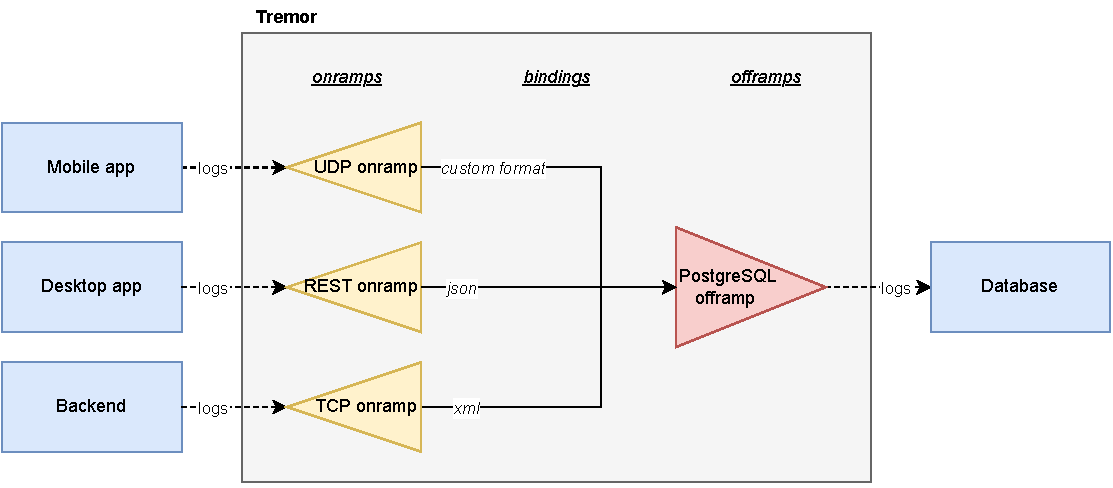
\includegraphics[width=\textwidth]{./Imagenes/example.pdf}
    \caption{Ejemplo de uso básico de Tremor}%
    \label{fig:tremor_example}
\end{figure}

Sin embargo, este caso subestima el potencial de Tremor. La entrada y salida del
sistema se pueden abstraer más, por ejemplo implementando un chatbot que
reproduce música. Este podría tomar mensajes de Discord como su entrada, y
enviar comandos con el API de Spotify como salida.

\section{Conceptos básicos}

Tremor se basa en los términos de \onramps o \sources y \offramps o \sinks:

\begin{itemize}
    \item Una \onramp especifica cómo Tremor se conecta con el mundo exterior (o
        una \pipeline) para \textbf{recibir} de sistemas externos. Por ejemplo
        TCP, periódicamente o PostgreSQL~\cite{tremoronramps}.

    \item Una \offramp especifica cómo Tremor se conecta con el mundo exterior
        (o una \pipeline) para \textbf{enviar} a sistemas externos. Por ejemplo,
        \emph{stdout}, Kafka o ElasticSearch~\cite{tremorofframps}.

    \item Una \pipeline es una lista de operaciones (transformación, agregación,
        eliminación, etc) a través de la cual se pueden encaminar los
        eventos~\cite{tremorpipelines}. La Figura \ref{fig:tremor_pipeline}
        muestra un ejemplo de una \pipeline, definida con Troy, su propio
        lenguaje inspirado en SQL.

\end{itemize}

TODO: mover lo siguiente al anexo y mencionar el leerlo para más detalles?

\begin{figure}
    \centering
    \begin{minted}[escapeinside=||]{mysql}
|\textcolor{blue}{define pipeline}| main
# The exit port is not a default port, so we have to overwrite the
# built-in port selection
into |out, exit|
|\textcolor{blue}{pipeline}|
  # Use the `std::string` module
  use std::|string|;
  use lib::scripts;

  # Create our script
  create |\textcolor{blue}{script}| punctuate from scripts::punctuate;

  # Filter any event that just is `"exit"` and send it to the exit port
  select {"graceful": false} from |in| where event == "exit" into |exit|;

  # Wire our capitailized text to the script
  select |string|::capitalize(event) from |in| where event != "exit"
    into punctuate;
  # Wire our script to the output
  select event from punctuate into |out|;
end;
    \end{minted}
    \caption{Ejemplo de una \pipeline definida para Tremor}%
    \label{fig:tremor_pipeline}
\end{figure}

Estos \onramps u \offramps suelen contener una cantidad de información que es
demasiado grande como para guardarla y debería tratarse en tiempo real. Su
procesado se basa en las siguientes operaciones:

\begin{itemize}
    \item \emph{Filtros}: descarte de eventos completos a partir de reglas
        configuradas, con el objetivo de eliminar información de la \pipeline
        que no se considera relevante.

    \item \emph{Transformaciones}: conversión de los datos de un formato a otro,
        así como incrementar un campo con un contador, reemplazar valores, o
        reorganizar su estructura.

    \item \emph{Matching}: búsqueda de partes de los eventos que siguen un
        patrón en específico (e.g., un campo \code{"id"} con un valor númerico)
        para transformarlo o descartarlo.

    \item \emph{Agregación} o \emph{rollups}: recolección de múltiples eventos
        para producir otros nuevos (e.g., la media o máximo de un campo), de
        forma que la información útil se reduzca en tamaño.

\end{itemize}

Finalmente, otros términos misceláneos sobre Tremor:

\begin{itemize}
    \item \emph{Códec}: describen cómo decodificar los datos del flujo y como
        volverlos a codificar. Por ejemplo, si los eventos de entrada usan JSON,
        tendrá que especificarse ese códec para que lo pueda entender Tremor.

    \item \emph{Preprocesador} o \emph{postprocesador}: operadores sobre flujos
        de datos brutos. Un preprocesador aplicará esta operación antes del
        códec y un postprocesador después. Por ejemplo, \code{base64} codifica o
        decodifica la información con ese protocolo.

    \item \emph{Artefacto}: término genérico para hablar de \sinks, \sources,
        códecs, preprocesadores y postprocesadores.

\end{itemize}

Para más información sobre Tremor se puede consultar \textcite{tremorintro}, que
introduce sus conceptos más básicos y sus posibles usos --- o cuándo \emph{no}
usarlo, en \textcite{tremorconstraints}. \textcite{tremorrecipes} lista un total
de 32 ejemplos de cómo configurar y emplear el software.

\section{Conectores}

Sin embargo, es posible que algunas \onramps no solo quieran recibir de sistemas
externos, sino también responderles directamente, actuando como una \offramp y
viceversa. Esto es especialmente útil para casos como REST y \websockets, donde
el protocolo da la posibilidad de responder a eventos, por ejemplo con un ACK,
usando la misma conexión. En la versión 0.11 --- la presente cuando me uní al
proyecto --- este problema se solucionaba con el concepto de \emph{linked
transports}.

El término \emph{conector} se introdujo en mayo de 2022 con la versión 0.12.
Solucionan el problema desde el inicio, abstrayendo tanto los \onramps como los
\offramps bajo el mismo concepto, incluyendo los \emph{linked transports}. Dado
que estos ya estaban siendo desarrollados mientras 0.11 era la última versión,
el sistema de plugins se enfocó a conectores desde el principio, en lugar de
\onramps u \offramps, que actualmente están en desuso.

A nivel de implementación, los conectores se definen con el \trait
\rust{Connector}, incluido en la figura \ref{fig:tremor_connector_trait}.
Esencialmente, los plugins de tipo conector exportarán públicamente esta
interfaz en su binario, y la runtime deberá ser capaz de cargarlo dinámicamente.
Actualmente, todos los conectores disponibles se listan y cargan de forma
estática al inicio del programa.

Por tanto, es importante mantener la interfaz de plugins lo más simple posible.
Los detalles de comunicación deberían dejarse a la runtime, de forma que los
plugins se limiten a exportar una lista de funciones síncronas. De esta forma,
se podrá evitar pasar tipos complejos (\rust{async}, canales de comunicación,
etc) entre la runtime y los plugins, que implicaría una carga de trabajo mucho
más alta.

Una vez esta interfaz de bajo nivel se defina, se puede crear un \emph{wrapper}
de más alto nivel en la runtime que se encargue de la comunicación y de mejorar
su usabilidad dentro de Tremor. Esto mismo lo hacen otras \crates como
\cratelink{rdkafka}, que implementa una capa de abstracción asíncrona sobre su
interfaz de C en \cratelink{rdkafka-sys}.

% vim: spelllang=es

\chapter{Validación experimental}

Lorem ipsum dolor sit amet, consectetuer adipiscing elit. Aenean commodo ligula eget dolor. Aenean massa. Cum sociis natoque penatibus et magnis dis parturient montes, nascetur ridiculus mus. Donec quam felis, ultricies nec, pellentesque eu, pretium quis, sem. Nulla consequat massa quis enim. Donec pede justo, fringilla vel, aliquet nec, vulputate eget, arcu. In enim justo, rhoncus ut, imperdiet a, venenatis vitae, justo. Nullam dictum felis eu pede mollis pretium. Integer tincidunt. Cras dapibus. Vivamus elementum semper nisi. Aenean vulputate eleifend tellus. Aenean leo ligula, porttitor eu, consequat vitae, eleifend ac, enim. Aliquam lorem ante, dapibus in, viverra quis, feugiat a, tellus. Phasellus viverra nulla ut metus varius laoreet. Quisque rutrum. Aenean imperdiet. Etiam ultricies nisi vel augue. Curabitur ullamcorper ultricies nisi. Nam eget dui. Etiam rhoncus. Maecenas tempus, tellus eget condimentum rhoncus, sem quam semper libero, sit amet adipiscing sem neque sed ipsum. Nam quam nunc, blandit vel, luctus pulvinar, hendrerit id, lorem. Maecenas nec odio et ante tincidunt tempus. Donec vitae sapien ut libero venenatis faucibus. Nullam quis ante. Etiam sit amet orci eget eros faucibus tincidunt. Duis leo. Sed fringilla mauris sit amet nibh. Donec sodales sagittis magna. Sed consequat, leo eget bibendum sodales, augue velit cursus nunc,

\ref{tab:etiqueta_tabla}

\begin{table}[!h]
\centering
\begin{tabular}{|c|c|c|}
\hline
Alumnos & Media & \multicolumn{1}{l|}{Nota} \\ \hline
Pérez  & 3,4                        & Suspenso           \\ \hline
Azaña  & 8,7                        & Notable          \\ \hline
\end{tabular}
\caption{Pie de tabla}
\label{tab:etiqueta_tabla}
\end{table}


% vim: spelllang=es

\chapter{Conclusiones y trabajo futuro}

\section{Concusiones}

La complejidad del proyecto ha resultado ser mucho mayor de lo esperado,
principalmente por el malentendido sobre la estabilidad del ABI de Rust. Por
tanto, ha resultado imposible desarrollar en el tiempo disponible un sistema de
plugins tan completo y eficiente como se especificaba inicialmente.

El problema principal tiene que ver con el rendimiento. Dada la naturaleza de
Tremor, es un requerimiento imprescindible para poderlo incluir en producción.
Tras las pruebas realizadas en el Anexo~\ref{annex:benchmarks}, se ha calculado
que el sistema de plugins reduce el rendimiento un 30\%.

No obstante, la última versión del sistema de plugins es perfectamente funcional
y, mediante su investigación, el diseño de su arquitectura y contribuciones de
código abierto, se ha hecho posible su inclusión en una futura versión de
Tremor.

Parte de esta ralentización en el desarrollo se debe también a Rust. Al ser un
lenguaje tan inmaduro es frecuente encontrar documentación pobre o librerías
incompletas. Muchas de las \crates usadas no disponían inicialmente de la
funcionalidad necesaria para un sistema de plugins, como \code{async_ffi},
\code{abi_stable}, \code{halfbrown} o \code{simd-json}. Se han resuelto
problemas importantes en el entorno, extendiendo el soporte para el ABI de C,
resolviendo tipos con varianzas inflexibles y elaborando conversiones de tipos
no triviales, todo ello manteniendo la máxima seguridad y eficiencia posible.
Con esfuerzos como estos, el desarrollo de proyectos similares en el futuro
resultará mucho más accesible.

\section{Futuro}

Se ha documentado tanto el proceso seguido como lo que queda pendiente, de forma
que el equipo de Tremor pueda continuar trabajando en el sistema de plugins para
su futuro lanzamiento. Sin embargo, aun después de esto el PDK nunca parará de
evolucionar: su uso se extenderá en la base de código y se perfeccionarán otras
características con el tiempo. Algunas ideas son las siguientes:

\begin{itemize}
    \item \textbf{Mejoras de rendimiento}: el enfoque principal para el primer
        lanzamiento del PDK. Esto incluye la realización de \emph{benchmarks}
        más variados y realistas, y el soporte de \abistable en más librerías.

    \item \textbf{Soporte de otros componentes de Tremor}: el PDK únicamente se
        implementa para los conectores, pero también podría funcionar con
        códecs, preprocesadores, postprocesadores, operadores, funciones,
        extractores, etc.

    \item \textbf{Refinamiento de la experiencia de usuario}: creación de
        proyectos modelo como base para plugins nuevos, ejemplos de uso, macros,
        documentación exhaustiva y de más alto nivel, frameworks de testing,
        etc.

    \item \textbf{Carga de plugins a petición del usuario}: además de poder
        cargar los plugins al inicio del programa, sería especialmente útil
        solicitar su carga durante la ejecución. Se podría elaborar un nuevo
        método de configuración iterativo, en el que se cargan y configuran los
        plugins uno a uno, y finalmente se exporta la composición final.

    \item \textbf{Paquetes de plugins}: en ciertos casos, sería más conveniente
        exportar un plugin que implemente más de un componente. Por ejemplo,
        podrían juntarse los conectores de TCP y UDP en único plugin, dado que
        probablemente compartan partes de su código y dependencias.

    \item \textbf{Gestión de versiones alternativas}: la implementación de
        \abistable para comprobar las versiones es rudimentaria y poco
        eficiente; se limita a comprobarlos todos recursivamente. Otra opción
        más simple sería únicamente comprobar una cadena con el versionado
        global para la interfaz, por ejemplo.

    \item \textbf{Mayor seguridad}: el cargado dinámico no ofrece ningún tipo de
        aislamiento sobre los plugins y no es adecuado si estos no son de
        confianza. Si en una futura versión de WebAssembly su rendimiento
        mejorase considerablemente, se podría volver a considerar su uso.

    \item \textbf{Registro centralizado de plugins}: en el futuro a largo plazo,
        se podría desarrollar una funcionalidad similar a los repositorios de
        Maven o Cargo. Allí se podrían guardar todos los plugins de la comunidad
        para gestionarlos automáticamente.

    \item \textbf{Eliminación de plugins en tiempo de ejecución}: es
        especialmente complejo de implementar, dado que \abistable
        explícitamente no lo soporta. Sin embargo, esto mejoraría
        considerablemente la resiliencia a errores, siendo posible reiniciar
        plugins completamente.

\end{itemize}

\section{Valoración personal}

Pese a las situaciones de frustración frente a todos los errores y bloqueos que
he encontrado en el camino, ha sido una experiencia extraordinaria. Matthias
bromeó una vez con que ``El infierno de debugging es importante para el
desarrollo de personaje'', y creo que tiene toda la razón. Enfrentarme a errores
que no sabía ni cómo abordar me ha enseñado mucho sobre Rust, y lo que es más
importante, sobre desarrollo de software en general.

Estoy muy satisfecho con haber conseguido lo que he conseguido, y aún más por
haberlo poder hecho junto al increíble equipo que es el de Tremor. Trabajar con
ellos me ha ayudado a descubrir qué quiero hacer tras la graduación, y con qué
tipo de empresa y personas quiero trabajar. Me mantendré en contacto con ellos
para seguir el progreso del sistema de plugins.


% BIBLIOGRAFÍA Y REFERENCIAS

\printbibliography%
\nocite{*} % Include all the entries in the bibliography, even if not mentioned

\newpage
\renewcommand\listfigurename{Lista de Figuras}
\listoffigures

\newpage
\renewcommand\listtablename{Lista de Tablas}
\listoftables

% ANEXOS

\newpage
\appendix
\clearpage
\addappheadtotoc%
\appendixpage%
\chapter{Guía de Rust}\label{annex:rust}

Es posible que en este anexo se omitan algunos conceptos o que algunas
explicaciones no sean completamente precisas por razones de simplicidad.
\namecite{rustbook} es el libro oficial para aprender Rust por completo, pero es
una lectura larga y posiblemente demasiado exhaustiva. Para mayor brevedad, se
recomienda leer \namecite{rustprofessionals}, \namecite{rustgentleintro} o
\namecite{rust30min}.

La comunidad dispone de otros libros que explican aspectos más avanzados del
lenguaje en específico, como \unsafe o la programación asíncrona. En esos casos,
se recomienda leer \namecite{nomicon} y \namecite{rustasyncbook},
respectivamente.

\section{Primeros pasos}

Comenzando por el clásico ``Hola Mundo'', se incluyen algunos ejemplos de cómo
es la sintaxis de Rust más básica. Los binarios o librerías en Rust reciben el
nombre de \crate. Nuestra \crate se podría ejecutar fácilmente con \emph{Cargo},
el administrador de dependencias oficial, o específicamente con el comando
\code{cargo run}.

\begin{minted}{rust}
fn main() {
    println!("Hello World!");
}
\end{minted}

\code{main} es nuestra función principal, que invoca al macro \code{println!}
para escribir por pantalla. Notar que la invocación de macros, a diferencia de
funciones, requiere un \rust{!} al final.

\section{Conceptos principales}

Los bloques básicos (\rust{if}, \rust{else}, \rust{while}, \rust{for}) son muy
similares a en otros lenguajes. También existe \rust{match}, que permite extraer
patrones de variables.

\begin{minted}{rust}
fn factorial(i: u64) -> u64 {
    match i {
        // Primer caso: i = 0
        0 => 1,
        // El resto de casos, asignado a una variable `n`
        n => n * factorial(n-1)
    }
}
\end{minted}

Uso de variables y métodos:

\begin{minted}{rust}
fn main() {
    // Declaración de una variable, cuyo tipo se infiere
    // automáticamente.
    let my_number = 1234;
    // Declaración de una variable con un tipo especificado
    // manualmente. Notar que se puede usar el mismo nombre, y la
    // variable anterior será destruida.
    let my_number: i32 = 4321;
    // Invocación de la función estática (constructor) `new` dentro
    // del tipo `String`. El uso de `mut` indica que la instancia del
    // tipo se puede modificar. Funciona de forma inversa a C++, que
    // por defecto es mutable y `const` indica que *no* se puede
    // modificar.
    let mut my_str = String::new();
    // Invocación del método `push` de `my_str`, que añade un
    // carácter al final de la cadena.
    my_str.push('a');
}
\end{minted}

Otros componentes principales de Rust son:

\begin{itemize}
    \item Estructuras de datos:

\begin{minted}{rust}
struct MessageA {
    // Campo público con una cadena de caracteres
    pub text: String,
    // Campo privado con un entero
    user_id: i32,
}
\end{minted}

\begin{minted}{rust}
// Sin nombres de campos; se pueden acceder con `data.0`
// y `data.1`, respectivamente.
struct MessageB(pub String, i32);
\end{minted}

    \item Enumeraciones, que también permiten contener datos:

\begin{minted}{rust}
enum MessageC {
    Join,
    Text(String, i32),
    Leave(i32),
}
\end{minted}

    \item \emph{Traits}, similares a las interfaces de Java en el sentido de que
        son una serie de requerimientos y que un tipo puede implementar
        múltiples \traits, pero también permiten implementaciones por defecto:

\begin{minted}{rust}
trait Sender {
    // Los métodos requieren especificar `self` explícitamente,
    // que es lo mismo que `this` en Java o C++. En este caso,
    // `&send` tomará una referencia al tipo que implemente
    // `Sender`. También podría ser una referencia mutable con
    // `&mut self`, o el mismo tipo con `self`.
    fn send(&self, msg: String);

    // Implementación por defecto.
    fn send_twice(&self, msg: String) {
        self.send(msg);
        self.send(msg.clone());
    }
}
\end{minted}

        Y para implementar un trait para un tipo:

\begin{minted}{rust}
impl Sender for MessageC {
    fn send(&self, msg: String) {
        match self {
            Join => println!("Joined"),
            Text(txt, id) => println!("{} sent: {}", id, txt),
            // Las variables `_` son ignoradas
            Leave(_) => println!("Left"),
        }
    }

    // `send_twice` se implementará automáticamente.
}
\end{minted}

    Notar que, sin embargo, Rust no es un lenguaje orientado a objetos. Un
    \trait puede heredar de otro \trait, pero un \struct no puede heredar de
    otro \struct.

\end{itemize}

\section{Genéricos y librería estándar}

De forma similar a C++, Rust posee tipos genéricos. Esto permite la
implementación de una librería estándar flexible, con varias estructuras de
datos importantes a conocer:

% NOTE: esto creo que lo puedo evitar si no incluyo cómo se usa async_ffi, que
% me parece demasiado complejo para el documento.
% \begin{minted}{rust}
% // Función genérica, donde `ToString` es un trait
% fn print<T: ToString>(t: T) {}

% // Otra manera de especificar genéricos con diferencias
% // menores que no se explicarán en esta introducción.
% fn print(t: impl ToString) {}
% \end{minted}

\begin{itemize}
    \item Tipos primitivos:
        \begin{itemize}
            \item Carácteres con \rust{char}.

            \item Punto flotante con \rust{f32} y \rust{f64}.

            \item Booleanos con \rust{bool}.

            \item Enteros: \rust{u8}, \rust{i8}, \rust{u16}, \rust{i16},
                \rust{u32}, \rust{i32}, \rust{u64}, \rust{i64}, e incluso
                \rust{i128} y \rust{u128} en las arquitecturas que lo soportan.

            \item Vectores de tamaño fijo: por ejemplo \rust{[1, 2, 3, 4, 5]}.

            \item N-tuplas como \rust{(1, true, 9.2)}.

            \item El tipo ``unidad'', \rust{()}, equivalente a \code{void} en C
                o C++.

            \item Punteros básicos con \rust{*const T} o \rust{*mut T}.

        \end{itemize}

    \item \rust{Vec<T>} representa un vector contiguo y redimensionable.

    \item \rust{HashMap<K, V>} es una tabla hash, genérica respecto a su clave
        \rust{K} y su valor \rust{V}. No se encuentra en el preludio, por lo que
        requeriría la siguiente declaración, similar a un \code{import} de Java:

\begin{minted}{rust}
use std::collections::HashMap;
\end{minted}

    \item \rust{Box<T>}, usado para localizar un tipo \rust{T} no nulo en
        memoria. Además de un \rust{*const T}, incluye el tamaño que ocupa
        \rust{T} y tiene una interfaz limitada para que su uso sea siempre
        seguro.

    \item \rust{str} es una cadena UTF-8 de solo lectura, típicamente usada con
        una referencia \rust{&str}. Va acompañada por su longitud, por lo que no
        hace falta terminarla con \code{\0}, a diferencia de C. \rust{String} es
        su versión modificable asignada en memoria.

\end{itemize}

\section{Gestión de errores}

En Rust, los errores se indican con el tipo \rust{Result<T, E>}. Este se trata
de una enumeración cuyo valor puede ser \rust{Ok(T)}, con el resultado obtenido
satisfactoriamente, o \rust{Err(E)}, con el tipo de error que ha sucedido. Dado
que el resultado está contenido dentro suyo, es imposible olvidar comprobar si
se ha producido algún error. Se puede usar \rust{match} para comprobar el
resultado, o una serie de funciones disponibles para hacer el proceso más
ergonómico:

\begin{minted}{rust}
match load_file(input) {
    Ok(data) => /* ... */,
    Err(e) => eprintln!("Error: {e}"),
}
\end{minted}

En caso de que se produjera un error del que el programa no se puediera
recuperar, como quedarse sin memoria o un fallo inesperado en la implementación,
se usa la funcionalidad de \emph{pánicos}. Un pánico se propaga de forma similar
a una excepción de C++ o Java, y terminará la ejecución por completo. Se puede
invocar con el macro \rust{panic!} o utilidades similares.

\section{Macros}

Rust cuenta con dos tipos de macros: \emph{declarativos} y \emph{procedurales}.
Ambos permiten generar código a tiempo de compilación, pero se diferencian
principalmente en la flexibilidad que ofrecen, a coste de un coste de desarrollo
menor o mayor, respectivamente.

Los macros declarativos se crean con una sintaxis especializada, similar a un
\rust{match} con patrones de tokens (identificadores, tipos, etc) como entrada,
y los tokens nuevos como salida. Son similares a los macros de C o C++, pero más
potentes e higiénicos (i.e., su expansión no captura identificadores
accidentalmente).

Los macros procedurales se describen como extensiones del lenguaje.
Esencialmente, ejecutan código en la compilación que consume y produce sintaxis
de Rust; consisten en directamente transformar el Árbol de Sintaxis Abstracta
(AST)~\cite[Procedural Macros]{rustref}. Consecuentemente, su complejidad es
mucho mayor, pero expanden las posibilidades de los macros enormemente.

\begin{minted}{rust}
some_macro!(1, 2, 3); // Puede ser tanto declarativo como procedural
\end{minted}

\begin{minted}{rust}
// Sintaxis típica de invocación de un macro
some_macro! {
    fn some_function() { /* ... */ }
}

// También permitido en el caso de los procedurales
#[some_macro]
fn some_function() { /* ... */ }
\end{minted}

Finalmente, los macros procedurales se pueden declarar de forma que
\emph{deriven} (implementen automáticamente) un \trait. Esto evita escribir
código repetitivo de forma muy sencilla:

\begin{minted}{rust}
// Con un macro `derive` para el trait `Debug`, que sirve para
// mostrar variables por pantalla.
#[derive(Debug)]
struct X(i32);

// Sin ellos sería lo siguiente. Como es trivial se puede
// simplificar en un macro procedural de tipo `derive`.
impl fmt::Debug for X {
    fn fmt(&self, f: &mut fmt::Formatter) -> fmt::Result {
        write!(f, "{:?}", self.0)
    }
}
\end{minted}

\section{Lifetimes}

La seguridad que provee Rust en memoria se basa en un modelo a tiempo de
compilación con \lifetimes. Una \lifetime es 

TODO: esto depende de cómo se acaba incluyendo la sección de ``problemas con
varianza y subtipado''.

\section{Unsafe}

Para poder mantener control completo a bajo nivel, es posible ignorar sus
garantías de seguridad con el sub-lenguaje llamado \emph{unsafe Rust}. El
análisis estático de Rust es conservativo; en algunas ocasiones es posible que
rechace algunos programas correctos. El desarrollador puede indicar que es
consciente de la situación y puede apagar este análisis para corregirlo por sí
mismo, arriesgándose a cometer un error en su código.

Se puede acceder a \emph{unsafe Rust} conteniendo el código dentro de un bloque
\rust{unsafe { /* ... */ }} o una función \rust{unsafe fn name() { /* ... */ }}.
Funciona igual que rust, pero incluye varias nuevas habilidades, entre otras:

\begin{itemize}
    \item Leer un puntero bruto en memoria

    \item Acceder o modificar una variable estática mutable

    \item Llamar a una función \unsafe

\end{itemize}

\section{Programación asíncrona}

Como muchos lenguajes modernos, Rust da soporte a la programación asíncrona, un
modelo de programación concurrente. Sin entrar en excesivo detalle, esta permite
tener una gran cantidad de \emph{tareas} concurrentes ejecutándose sobre unos
pocos hilos del Sistema Operativo. Su caso de uso principal es programas cuyo
rendimiento está limitado por operaciones de entrada y salida, como servidores o
bases de datos~\cite{rustasyncbook}.

\begin{minted}{rust}
// Con `async` se indica que la función es asíncrona.
async fn get_two_sites_async() {
    // Creación de dos "futuros" que, al completarse, descargarán
    // asíncronamente las páginas web. Similar a la creación de
    // un nuevo hilo.
    let future_one = download_async("https://www.foo.com");
    let future_two = download_async("https://www.bar.com");

    // Ejecutar las dos tareas. Similar a esperar la terminación de
    // los hilos.
    join!(future_one, future_two);

    // Con `.await` se puede esperar a la terminación de un futuro
    // individual.
    let future_three = download_async("https://www.bar.com").await;
}
\end{minted}



\end{document}
